\documentclass[12pt]{article}
\usepackage[a4paper, margin=1in]{geometry}
\usepackage{titlesec}
\usepackage{hyperref}
\usepackage{graphicx}
\usepackage{enumitem}
\usepackage{float}
\titleformat{\section}[block]{\large\bfseries}{\thesection.}{0.5em}{}
\titleformat{\subsection}[block]{\normalsize\bfseries}{\thesubsection.}{0.5em}{}


\title{Software Requirements Specification\\\large\textbf{Mavito Multilingual Terminology PWA}}
\author{Team Name: Velox}
\date{\today}

\begin{document}

\maketitle
\tableofcontents
\newpage

\section{Introduction}
\subsection{Purpose}
The purpose of this document is to define the software requirements of the Mavito system, a multilingual terminology web application developed as part of the COS 301 Capstone project at the University of Pretoria. This document is intended to guide the development team, ensure alignment with client expectations, and serve as a reference for future maintenance, testing, and extension of the platform.

\subsection{Scope}
Mavito is a multilingual, progressive web application (PWA) designed to provide users with access to curated statistical terminology in all 11 official South African languages. The system enables users to search and browse glossary terms, submit suggestions, and engage through a gamified contribution model. Mavito supports offline functionality, glossary versioning, contributor uploads, and plugin-based feature extensions including AI-enhanced semantic search and analytics. The system is built using a microkernel-microservices architecture for flexibility, modularity, and future extensibility.

\subsection{Intended Audience}
This document is primarily intended for:
\begin{itemize}
    \item \textbf{Developers and engineers} responsible for implementing and maintaining the system.
    \item \textbf{Project stakeholders and academic supervisors} overseeing the design, quality, and alignment of Mavito with its educational goals.
    \item \textbf{Testers and QA personnel} who require a clear specification of expected system behavior.
    \item \textbf{Future contributors} who may extend the application or onboard new glossaries and features.
\end{itemize}

\subsection{Document Overview}
The remainder of this document includes detailed user stories, functional and non-functional requirements, architectural and design patterns, service contracts, constraints, and system models. It is structured to follow industry best practices and academic guidelines for software specification documents, ensuring clarity and completeness for all stakeholders.

\subsection{Definitions, Acronyms, and Abbreviations}
\begin{itemize}
    \item \textbf{PWA}: Progressive Web Application
    \item \textbf{CI/CD}: Continuous Integration and Continuous Deployment
\end{itemize}


\section{User Stories}
This section outlines the high-level user goals and core system interactions that informed the functional requirements. Detailed use case specifications and diagrams can be found in the official project repository.

\subsection{User Story \#1: Sync Updates}

\textbf{ID:} US001 (Mavito Project) \\
\textbf{Title:} Automatic Synchronization of Downloaded Lexicon Data \\
\textbf{As a:} Mavito application user (e.g., language enthusiast, NLP researcher, student) who has downloaded lexicon data for offline use, \\
\textbf{I want:} the application to automatically check for and apply updates to my downloaded lexicon data whenever I am online, \\
\textbf{So that:} I can be confident that I am always working with the most current and accurate version of the linguistic information without needing to manually re-download or check for updates.

\vspace{1em}
\textbf{Acceptance Criteria:}
\begin{enumerate}
    \item \textbf{Automatic Update Check:}
    \begin{itemize}
        \item \textbf{Given} I have previously downloaded lexicon data,
        \item \textbf{And} I open the Mavito application with an active internet connection,
        \item \textbf{Then} the application automatically initiates a check for updates to my downloaded data against the central repository in the background.
    \end{itemize}

    \item \textbf{Notification of Available Updates (Recommended):}
    \begin{itemize}
        \item \textbf{Given} updates are available for my downloaded data,
        \item \textbf{Then} the application clearly notifies me that updates are available (e.g., via a subtle in-app notification, a badge on a settings icon).
        \item \textbf{And} the notification provides an option to view details about the updates (e.g., number of terms changed, lexicon version).
    \end{itemize}

    \item \textbf{Update Process:}
    \begin{itemize}
        \item \textbf{Given} updates are available and I have an active internet connection,
        \item \textbf{Then} the application allows me to initiate the download and application of these updates (or this happens automatically, depending on user settings or application design).
        \item \textbf{And} the application provides clear feedback on the progress of the update (e.g., download progress bar, installation status).
        \item \textbf{And} the update process is efficient and minimizes data usage (e.g., by only downloading changes/deltas if possible, rather than the entire dataset, for future enhancements).
    \end{itemize}

    \item \textbf{Successful Update:}
    \begin{itemize}
        \item \textbf{Given} the update process completes successfully,
        \item \textbf{Then} my locally stored lexicon data reflects the latest version from the central repository.
        \item \textbf{And} I receive a confirmation message that the data has been updated.
    \end{itemize}

    \item \textbf{Handling No Updates:}
    \begin{itemize}
        \item \textbf{Given} I am online and no updates are available for my downloaded data,
        \item \textbf{Then} the application does not interrupt my workflow with unnecessary notifications (or provides a subtle indication that data is ``up-to-date'').
    \end{itemize}

    \item \textbf{Offline State Post-Sync:}
    \begin{itemize}
        \item \textbf{Given} my data has been successfully synced,
        \item \textbf{Then} the newly updated data is fully accessible offline.
    \end{itemize}

    \item \textbf{Error Handling - Interrupted Connection:}
    \begin{itemize}
        \item \textbf{Given} an update is in progress and my internet connection is lost,
        \item \textbf{Then} the application gracefully pauses or stops the update process.
        \item \textbf{And} I am notified of the interruption.
        \item \textbf{And} the application attempts to resume the update when the connection is re-established, or allows me to manually retry.
        \item \textbf{And} my previously downloaded (pre-update attempt) data remains intact and usable.
    \end{itemize}

    \item \textbf{Error Handling - Sync Conflict (Advanced Consideration for Future):}
    \begin{itemize}
        \item \textbf{Given} a conflict occurs during synchronization (e.g., if local modifications were possible vs. server changes),
        \item \textbf{Then} the system has a defined strategy for conflict resolution (e.g., prioritizes server version for this project's scope, notifies user if manual intervention were ever needed).
    \end{itemize}

    \item \textbf{User Control (Optional Enhancement):}
    \begin{itemize}
        \item \textbf{Given} I am a user concerned about data usage or update timing,
        \item \textbf{Then} I may have an option in settings to control sync behavior (e.g., sync only on Wi-Fi, schedule syncs, manual sync only).
    \end{itemize}
\end{enumerate}

\vspace{1em}
\textbf{Notes/Assumptions:}
\begin{itemize}
    \item This user story assumes that users primarily download data for offline reading and searching. Contributions and comments are made while online and sent to a central repository (as per Functional Requirement FR4.3).
    \item The complexity of only downloading changes/deltas (Acceptance Criterion 3.4) can be significant. For an initial implementation, syncing entire updated files might be a simpler starting point, with delta updates as a future enhancement.
    \item Conflict resolution (Acceptance Criterion 8) is likely simplified if the local data is treated as a read-only cache that gets overwritten by server updates, which aligns with the current understanding of the Mavito project.
\end{itemize}



\subsection{User Story \#2: Download Language Resources for Offline Access}

\textbf{ID:} US002 (Mavito Project) \\
\textbf{Title:} Download Select Language Resources for Offline Use \\
\textbf{As a:} Mavito application user (e.g., language enthusiast, NLP researcher, student), \\
\textbf{I want:} to be able to select and download specific language resources (like individual lexicons, glossaries, or dictionaries) to my device, \\
\textbf{So that:} I can access and use this information even when I do not have an active internet connection.

\vspace{1em}
\textbf{Acceptance Criteria:}
\begin{enumerate}
    \item \textbf{Discover and Select Resources for Download:}
    \begin{itemize}
        \item \textbf{Given} I am browsing the available language resources within the application (while online),
        \item \textbf{Then} I can clearly identify which resources are available for download.
        \item \textbf{And} I can select one or more language resources to download.
        \item \textbf{And} the application shows the estimated size of the selected resource(s) before initiating the download.
    \end{itemize}

    \item \textbf{Initiate Download:}
    \begin{itemize}
        \item \textbf{Given} I have selected one or more language resources for download,
        \item \textbf{Then} I can initiate the download process with a clear action (e.g., a ``Download'' button).
    \end{itemize}

    \item \textbf{Download Process Feedback:}
    \begin{itemize}
        \item \textbf{Given} a download is in progress,
        \item \textbf{Then} the application provides clear visual feedback on the download status (e.g., progress bar, percentage complete, estimated time remaining).
        \item \textbf{And} I can continue to use other online features of the application while a download is in progress (background download).
        \item \textbf{And} I have the option to pause and resume a download if needed.
        \item \textbf{And} I have the option to cancel an ongoing download.
    \end{itemize}

    \item \textbf{Successful Download and Storage:}
    \begin{itemize}
        \item \textbf{Given} a language resource download completes successfully,
        \item \textbf{Then} the application notifies me that the download is complete.
        \item \textbf{And} the downloaded resource is stored locally on my device in a way that the Mavito application can access it offline.
        \item \textbf{And} the application clearly indicates which resources have been successfully downloaded and are available offline.
    \end{itemize}

    \item \textbf{Managing Downloaded Resources:}
    \begin{itemize}
        \item \textbf{Given} I have downloaded language resources,
        \item \textbf{Then} I can view a list of all my downloaded resources within the application.
        \item \textbf{And} I can remove/delete downloaded resources from my device to free up storage space.
        \item \textbf{And} the application shows the amount of local storage space currently used by downloaded Mavito resources.
    \end{itemize}

    \item \textbf{Error Handling - Insufficient Storage:}
    \begin{itemize}
        \item \textbf{Given} I attempt to download a resource,
        \item \textbf{And} my device has insufficient storage space,
        \item \textbf{Then} the application informs me of the insufficient storage and the download does not proceed (or pauses until space is freed).
    \end{itemize}

    \item \textbf{Error Handling - Interrupted Connection During Download:}
    \begin{itemize}
        \item \textbf{Given} a download is in progress and my internet connection is lost,
        \item \textbf{Then} the application gracefully pauses the download process.
        \item \textbf{And} I am notified of the interruption.
        \item \textbf{And} the application attempts to resume the download automatically when the connection is re-established, or allows me to manually resume.
    \end{itemize}

    \item \textbf{Error Handling - Download Failure:}
    \begin{itemize}
        \item \textbf{Given} a download fails for reasons other than connection loss or insufficient storage (e.g., server error, corrupted file),
        \item \textbf{Then} the application notifies me of the failure and provides a reason if possible.
        \item \textbf{And} I have the option to retry the download.
    \end{itemize}

    \item \textbf{Accessing Downloaded Resources Offline:}
    \begin{itemize}
        \item \textbf{Given} I have successfully downloaded a language resource,
        \item \textbf{And} I am offline,
        \item \textbf{Then} I can access and use that downloaded resource within the Mavito application.
    \end{itemize}
\end{enumerate}

\vspace{1em}
\textbf{Notes/Assumptions:}
\begin{itemize}
    \item The user must be online to browse and initiate downloads.
    \item The application will need appropriate permissions to write to local device storage.
    \item The format of the downloaded data should be optimized for offline use and efficient storage.
    \item This user story focuses on the \textit{download} functionality. A separate user story would cover the specifics of \textit{accessing and using} the data offline (e.g., offline search within downloaded resources).
\end{itemize}


\subsection{User Story \#3: Search Feature}

\textbf{ID:} US003 (Mavito Project) \\
\textbf{Title:} Multilingual Term Search \\
\textbf{As a:} Mavito application user (e.g., casual user, linguist, or contributor), \\
\textbf{I want:} to search across multiple multilingual glossaries and dictionaries using filters and smart suggestions, \\
\textbf{So that:} I can quickly find definitions, translations, and related entries in my preferred language.

\vspace{1em}
\textbf{Acceptance Criteria:}
\begin{enumerate}
    \item \textbf{Query Input:}
    \begin{itemize}
        \item \textbf{Given} I am on the main search page,
        \item \textbf{When} I enter a query into the search bar,
        \item \textbf{Then} the system searches across all selected data sources and returns matching terms.
    \end{itemize}

    \item \textbf{Filter Options:}
    \begin{itemize}
        \item \textbf{Given} I want to refine my search,
        \item \textbf{Then} I can apply filters like language, part of speech, or glossary type before or after submitting the query.
    \end{itemize}

    \item \textbf{Fuzzy Search (Optional):}
    \begin{itemize}
        \item \textbf{Given} my query has a typo or partial match,
        \item \textbf{Then} the system offers similar results using fuzzy matching.
    \end{itemize}

    \item \textbf{AI-Powered Suggestions (Optional):}
    \begin{itemize}
        \item \textbf{Given} I start typing in the search bar,
        \item \textbf{Then} I see AI-generated autocomplete suggestions based on common terms or semantic matches.
    \end{itemize}

    \item \textbf{Search History:}
    \begin{itemize}
        \item \textbf{Given} I have searched for terms in the past,
        \item \textbf{Then} the system shows my recent queries and allows re-searching them.
    \end{itemize}

    \item \textbf{Sorting and Result Presentation:}
    \begin{itemize}
        \item \textbf{Given} the results are displayed,
        \item \textbf{Then} I can sort them by relevance, alphabetical order, or popularity,
        \item \textbf{And} each result shows the term, language, and a brief definition snippet.
    \end{itemize}
\end{enumerate}

\vspace{1em}
\textbf{Assumptions:}
\begin{itemize}
    \item Offline support will allow previously downloaded glossaries to be searched.
    \item Filters and sort options persist across sessions.
    \item AI and fuzzy search are optional enhancements.
    \item Glossary datasets are already available and preloaded or fetched via sync.
\end{itemize}

\subsection{User Story \#4: Feedback Submissions}
\textbf{ID:} US004 (Mavito Project) \\
\textbf{Title:} User Contributions and Feedback \\
\textbf{As a:} logged-in user of the application, \\
\textbf{I want:} to be able to comment on terms and submit feedback or error reports, \\
\textbf{So that:} I can contribute to improving the accuracy and usefulness of the data content.

\vspace{1em}
\textbf{Acceptance Criteria:}
\begin{enumerate}
    \item \textbf{Commenting on Terms:}
    \begin{itemize}
        \item \textbf{Given} I am logged into my account,
        \item \textbf{And} I am viewing a term or entry,
        \item \textbf{Then} I should see a comment section below the entry,
        \item \textbf{And} I should be able to submit my own comment.
    \end{itemize}

    \item \textbf{Submitting Feedback:}
    \begin{itemize}
        \item \textbf{Given} I am logged into my account,
        \item \textbf{And} I am viewing a specific term or entry,
        \item \textbf{And} I choose to provide feedback,
        \item \textbf{Then} I should be presented with a feedback form,
        \item \textbf{And} I should receive a confirmation message after successfully submitting the feedback.
    \end{itemize}

    \item \textbf{Voting on User Contributions:}
    \begin{itemize}
        \item \textbf{Given} I am logged into my account,
        \item \textbf{And} I am viewing a comment or suggestion submitted by another user,
        \item \textbf{Then} I should see upvote and downvote buttons associated with it,
        \item \textbf{And} I should be able to cast one vote per contribution,
        \item \textbf{And} the vote count should update immediately after I vote.
    \end{itemize}

    \item \textbf{Approval Status of Feedback:}
    \begin{itemize}
        \item \textbf{Given} I have submitted feedback for a term,
        \item \textbf{And} the feedback has been approved by a moderator,
        \item \textbf{Then} the approved feedback should be integrated into the application content,
        \item \textbf{And} I should receive a notification confirming the integration.
    \end{itemize}

    \item \textbf{Marking Approved Submissions:}
    \begin{itemize}
        \item \textbf{Given} user feedback or content has been approved and integrated,
        \item \textbf{Then} the associated entry should be visibly marked as a ``User Submission'' to distinguish it from original content.
    \end{itemize}

    \item \textbf{Rewarding User Contributions (Optional Gamification):}
    \begin{itemize}
        \item \textbf{Given} I am logged in and submit a comment, feedback, or report,
        \item \textbf{When} my contribution meets a predefined threshold (e.g., approved, upvoted),
        \item \textbf{Then} I should earn points or badges for that action,
        \item \textbf{And} my contribution stats should be viewable in my profile.
    \end{itemize}
\end{enumerate}

\vspace{1em}
\textbf{Notes/Assumptions:}
\begin{itemize}
    \item Only logged-in users can comment, submit feedback, vote, or receive contribution rewards.
    \item Users must have verified accounts to interact with community features (e.g., comments, voting).
    \item Rate limiting will be implemented to prevent spam submissions.
\end{itemize}

\subsection{User Story \#5: Gamification Feature}

\textbf{ID:} US005 (Mavito Project) \\
\textbf{Title:} Contribution-Based Rewards and Progress Tracking \\
\textbf{As a:} frequent Mavito contributor (e.g., user who submits suggestions or comments), \\
\textbf{I want:} to earn points, unlock badges, and track my contribution progress, \\
\textbf{So that:} I feel motivated to participate and can see recognition for my efforts.

\vspace{1em}
\textbf{Acceptance Criteria:}
\begin{enumerate}
    \item \textbf{Points for Contribution:}
    \begin{itemize}
        \item \textbf{Given} I submit a suggestion, comment, or report an issue on a term,
        \item \textbf{Then} I earn points based on the type and quality of the contribution.
    \end{itemize}
    
    \item \textbf{Achievement Unlocking:}
    \begin{itemize}
        \item \textbf{Given} I reach a milestone,
        \item \textbf{Then} I unlock a badge or achievement.
    \end{itemize}

    \item \textbf{Progress Dashboard:}
    \begin{itemize}
        \item \textbf{Given} I navigate to my profile,
        \item \textbf{Then} I can view my total points, badges earned, and contribution rank.
    \end{itemize}

    \item \textbf{Real-Time Feedback:}
    \begin{itemize}
        \item \textbf{Given} I perform a gamified action,
        \item \textbf{Then} I receive instant feedback such as a pop-up message.
    \end{itemize}

    \item \textbf{Leveling Up:}
    \begin{itemize}
        \item \textbf{Given} I reach predefined thresholds,
        \item \textbf{Then} my user rank or title updates accordingly.
    \end{itemize}

    \item \textbf{Offline Support:}
    \begin{itemize}
        \item \textbf{Given} I contribute while offline,
        \item \textbf{Then} my contributions and points are synced once I reconnect.
    \end{itemize}
\end{enumerate}

\subsection{User Story \#6: UpVote System}

\textbf{ID:} US006 (Mavito Project) \\
\textbf{Title:} Crowdsourced Validation via UpVoting \\
\textbf{As a:} Mavito application user (e.g., casual user, linguist, or academic) who wants to contribute to the accuracy and quality of lexicon entries, \\
\textbf{I want:} to upvote (or downvote) suggested changes or comments on terms in the lexicon, \\
\textbf{So that:} the community can collectively validate contributions, and moderators can prioritize high-quality updates for integration into the central repository.

\vspace{1em}
\textbf{Acceptance Criteria:}
\begin{enumerate}
    \item \textbf{Voting Interface:}
    \begin{itemize}
        \item \textbf{Given} I am viewing a term entry with user-submitted comments or suggested changes,
        \item \textbf{Then} I see an option to upvote or downvote each contribution.
        \item \textbf{And} the current vote count is displayed next to each contribution.
    \end{itemize}

    \item \textbf{Vote Submission:}
    \begin{itemize}
        \item \textbf{Given} I am logged in and have not yet voted on a specific contribution,
        \item \textbf{When} I click the upvote/downvote button,
        \item \textbf{Then} my vote is recorded immediately (if online) or queued for sync (if offline).
        \item \textbf{And} the UI reflects my vote and updates the vote count.
    \end{itemize}

    \item \textbf{Prevent Duplicate Voting:}
    \begin{itemize}
        \item \textbf{Given} I have already voted on a contribution,
        \item \textbf{Then} the UI prevents me from voting again (unless I undo my vote).
    \end{itemize}

    \item \textbf{Offline Handling:}
    \begin{itemize}
        \item \textbf{Given} I vote while offline,
        \item \textbf{Then} the vote is stored locally and synced to the central repository when I reconnect.
    \end{itemize}

    \item \textbf{Moderation Visibility (Optional Enhancement):}
    \begin{itemize}
        \item \textbf{Given} I am a moderator,
        \item \textbf{Then} I can filter contributions by vote count to prioritize high-quality submissions.
    \end{itemize}

    \item \textbf{Feedback Transparency:}
    \begin{itemize}
        \item \textbf{Given} a contribution receives significant downvotes,
        \item \textbf{Then} the system may flag it for review (future enhancement).
    \end{itemize}
\end{enumerate}

\vspace{1em}
\textbf{Notes/Assumptions:}
\begin{itemize}
    \item Voting requires user authentication to prevent abuse.
    \item Vote counts are public to encourage transparency.
    \item Offline votes are treated as "pending" until synced.
    \item Future enhancements could include:
    \begin{itemize}
        \item Weighted voting for trusted users (e.g., linguists).
    \end{itemize}
\end{itemize}


\subsection{User Story \#7.1: Word Frequency Trends}

\textbf{ID:} US007.1 (Marito Project) \\
\textbf{Title:} Historical Word Usage Visualization \\
\textbf{As a:} Linguist or language researcher studying lexical evolution, \\
\textbf{I want:} To view historical trends of word usage frequency across different time periods, \\
\textbf{So that:} I can identify patterns in language adoption, obsolescence, or cultural influences.

\vspace{1em}
\textbf{Acceptance Criteria:}
\begin{enumerate}
    \item \textbf{Trend Visualization:}
    \begin{itemize}
        \item \textbf{Given} I select a word or phrase,
        \item \textbf{Then} I see a line chart showing its monthly/quarterly/yearly frequency.
        \item \textbf{And} can toggle between absolute counts and percentage changes.
    \end{itemize}

    \item \textbf{Comparative Analysis:}
    \begin{itemize}
        \item \textbf{Given} I select multiple words,
        \item \textbf{Then} the system overlays their trends with distinct colors.
        \item \textbf{And} provides a legend identifying each word.
    \end{itemize}

    \item \textbf{Contextual Data:}
    \begin{itemize}
        \item \textbf{Given} I hover over a data point,
        \item \textbf{Then} I see exact usage counts and sample sentences.
        \item \textbf{And} can click to view source documents.
    \end{itemize}

    \item \textbf{Export Functionality:}
    \begin{itemize}
        \item \textbf{Given} I want to analyze data externally,
        \item \textbf{Then} I can export charts as PNG or data as CSV/JSON.
    \end{itemize}
\end{enumerate}

\vspace{1em}
\textbf{Notes/Assumptions:}
\begin{itemize}
    \item Data aggregates nightly for performance.
    \item Supports all 12 official South African languages.
    \item Default view shows last 12 months.
    \item Future enhancements could include:
    \begin{itemize}
        \item Regional usage heatmaps.
        \item Sociolinguistic correlation analysis.
    \end{itemize}
\end{itemize}

\subsection{User Story \#7.2: Contribution Analytics}

\textbf{ID:} US007.2 (Marito Project) \\
\textbf{Title:} User Contribution Visualization \\
\textbf{As a:} Regular contributor to the Mavito platform, \\
\textbf{I want:} To see a breakdown of my edits and comments across languages, \\
\textbf{So that:} I can track my impact and focus on underrepresented languages.

\vspace{1em}
\textbf{Acceptance Criteria:}
\begin{enumerate}
    \item \textbf{Personal Dashboard:}
    \begin{itemize}
        \item \textbf{Given} I view my profile,
        \item \textbf{Then} I see a pie chart of my contributions by language.
        \item \textbf{And} a timeline of my activity.
    \end{itemize}

    \item \textbf{Progress Metrics:}
    \begin{itemize}
        \item \textbf{Given} I'm an active user,
        \item \textbf{Then} I see my percentile ranking in the community.
        \item \textbf{And} suggested languages needing more contributions.
    \end{itemize}
\end{enumerate}

\vspace{1em}
\textbf{Notes/Assumptions:}
\begin{itemize}
    \item Updates within 5 minutes of contributions.
    \item Includes all contribution types.
    \item Future enhancements could include:
    \begin{itemize}
        \item Team contribution tracking.
        \item Contribution quality scoring.
    \end{itemize}
\end{itemize}

\subsection{User Story \#7.3: Trending Terms}

\textbf{ID:} US007.3 (Marito Project) \\
\textbf{Title:} Real-Time Popularity Tracking \\
\textbf{As a:} Language learner or cultural researcher, \\
\textbf{I want:} To see which words are currently trending in popularity, \\
\textbf{So that:} I can stay current with evolving language usage.

\vspace{1em}
\textbf{Acceptance Criteria:}
\begin{enumerate}
    \item \textbf{Trending Display:}
    \begin{itemize}
        \item \textbf{Given} I visit the homepage,
        \item \textbf{Then} I see a ``Trending Now'' carousel with top terms.
        \item \textbf{And} percentage change indicators.
    \end{itemize}

    \item \textbf{Contextual Information:}
    \begin{itemize}
        \item \textbf{Given} I select a trending word,
        \item \textbf{Then} I see related news/events driving popularity.
        \item \textbf{And} its historical frequency graph.
    \end{itemize}
\end{enumerate}

\vspace{1em}
\textbf{Notes/Assumptions:}
\begin{itemize}
    \item Updates every 4 hours.
    \item Excludes spam/fake trends.
    \item Future enhancements could include:
    \begin{itemize}
        \item User-submitted trend explanations.
        \item Regional trend variations.
    \end{itemize}
\end{itemize}




\vspace{1em}
\textbf{Assumptions:}
\begin{itemize}
    \item Contributions are validated before points are awarded to prevent abuse.
    \item Gamification rewards are symbolic, not monetary.
    \item This feature is designed to encourage consistent, high-quality engagement.
\end{itemize}


\subsection{User Story \#8: Responsive Design}
\textbf{ID:} US008 (Marito Project) \\
\textbf{Title:} Responsive Layout for Mobile and Desktop Devices \\
\textbf{As a:} user who may need to access the Mavito application while on the go, \\
\textbf{I want:} the user interface to adapt and remain fully functional on mobile phones, tablets, and desktops, \\
\textbf{So that:} I can quickly and seamlessly use the application in any situation, regardless of the device I'm using.

\vspace{1em}
\textbf{Acceptance Criteria:}
\begin{enumerate}
    \item \textbf{Mobile Adaptability:}
    \begin{itemize}
        \item \textbf{Given} I am using the Mavito application,
        \item \textbf{And} I am on a mobile device,
        \item \textbf{Then} the layout should automatically adjust to fit the screen without horizontal scrolling.
    \end{itemize}

    \item \textbf{Touch-Friendly UI:}
    \begin{itemize}
        \item \textbf{Given} I am interacting with the app on a touchscreen device,
        \item \textbf{And} I tap on any button or link,
        \item \textbf{Then} the tapped element should be responsive to touch and have a minimum tap area of 48px × 48px.
    \end{itemize}

    \item \textbf{Touchscreen Swiping and Scrolling Support:}
    \begin{itemize}
        \item \textbf{Given} I am using the Mavito app on a touchscreen device,
        \item \textbf{And} I am viewing content that extends beyond the initial screen (e.g., a list or feed),
        \item \textbf{Then} I should be able to scroll vertically or horizontally (depending on the content) using swipe gestures,
        \item \textbf{And} the scrolling should be smooth and responsive.
    \end{itemize}

    \item \textbf{Adaptive Mobile Navigation Elements:}
    \begin{itemize}
        \item \textbf{Given} I am using the Mavito app on a mobile device,
        \item \textbf{Then} the navigation should adapt to a mobile-friendly layout, such as displaying a hamburger menu instead of a full-width navigation bar.
    \end{itemize}

    \item \textbf{Device Orientation Handling:}
    \begin{itemize}
        \item \textbf{Given} I am using the app on a mobile device,
        \item \textbf{And} I switch between portrait and landscape mode,
        \item \textbf{Then} the UI layout should follow without breaking or cutting off content.
    \end{itemize}

    \item \textbf{Mobile Hardware and OS Compatibility:}
    \begin{itemize}
        \item \textbf{Given} I am using the Mavito app on a mobile device running a supported OS (e.g., Android 10+, iOS 13+),
        \item \textbf{And} the device has at least 2 GB of RAM and a modern mobile browser (e.g., Chrome),
        \item \textbf{Then} all core features should work smoothly without crashes or performance lags.
    \end{itemize}

    \item \textbf{Error Handling - Network Errors (Mobile Use):}
    \begin{itemize}
        \item \textbf{Given} I lose internet connectivity due to a poor signal while using the app,
        \item \textbf{Then} the application should seamlessly switch to its offline version without interruption,
        \item \textbf{And} provide an indication informing me that the app is currently in offline mode.
    \end{itemize}
\end{enumerate}

\vspace{1em}
\textbf{Notes/Assumptions:}
\begin{itemize}
    \item Devices with screen widths less than or equal to 768 pixels are considered mobile, and touch interaction is expected on these devices.
\end{itemize}

\subsection{User Story \#9: Dictionary Term Display}
\textbf{ID:} US09 (Marito Project) \\
\textbf{Title:} Comprehensive Term Presentation \\
\textbf{As a:} user who has found a term through search, \\
\textbf{I want:} to view complete information about a specific term, \\
\textbf{So that:} I can understand its full definition and translations.

\vspace{1em}
\textbf{Acceptance Criteria:}
\begin{enumerate}
    \item \textbf{Definition Display:}
    \begin{itemize}
        \item \textbf{Given} I have selected a term from search results,
        \item \textbf{Then} I should see its complete definition,
        \item \textbf{And} its assigned category with clickable link to the full glossary.
    \end{itemize}

    \item \textbf{Translation Panel:}
    \begin{itemize}
        \item \textbf{Given} I am viewing a term,
        \item \textbf{Then} all available translations should be displayed in a structured table,
        \item \textbf{With} clear language code labels (e.g., "afr", "zul").
    \end{itemize}

    \item \textbf{Missing Data Handling:}
    \begin{itemize}
        \item \textbf{Given} a term lacks translation for certain languages,
        \item \textbf{Then} those fields should display "Translation not available",
        \item \textbf{And} be visually distinct from complete entries.
    \end{itemize}
\end{enumerate}

\vspace{1em}
\textbf{Notes/Assumptions:}
\begin{itemize}
    \item Integrates with US003 search results
    \item Preserves all existing search filters when navigating from results to term view
\end{itemize}

\subsection{User Story \#10: Glossary Category Navigation}
\textbf{ID:} US010 (Marito Project) \\
\textbf{Title:} Browse Terms by Subject Area \\
\textbf{As a:} user interested in exploring specific domains (e.g., Agriculture, Legal), \\
\textbf{I want:} to browse all terms within a particular category, \\
\textbf{So that:} I can discover related terminology.

\vspace{1em}
\textbf{Acceptance Criteria:}
\begin{enumerate}
    \item \textbf{Category Selection:}
    \begin{itemize}
        \item \textbf{Given} I access the glossary browser,
        \item \textbf{Then} I should see all available categories,
        \item \textbf{And} be able to sort them alphabetically or by term count.
    \end{itemize}

    \item \textbf{Term Listing:}
    \begin{itemize}
        \item \textbf{Given} I select a category (e.g., "Agriculture"),
        \item \textbf{Then} I should see paginated results of all terms,
        \item \textbf{With} options to filter by language availability.
    \end{itemize}

    \item \textbf{Cross-Referencing:}
    \begin{itemize}
        \item \textbf{Given} I view a term in a glossary,
        \item \textbf{Then} I should see related terms from the same category,
        \item \textbf{And} options to navigate to similar categories.
    \end{itemize}
\end{enumerate}

\vspace{1em}
\textbf{Notes/Assumptions:}
\begin{itemize}
    \item Categories are predefined based on dataset taxonomy
    \item Works both online and for downloaded glossaries
\end{itemize}

\subsection{User Story \#11: Term Bank Translations}
\textbf{ID:} US011 (Marito Project) \\
\textbf{Title:} Access Multilingual Translations \\
\textbf{As a:} multilingual user, \\
\textbf{I want:} to toggle between translations for a term, \\
\textbf{So that:} I can understand it in my preferred language.

\vspace{1em}
\textbf{Acceptance Criteria:}
\begin{enumerate}
    \item \textbf{Translation Toggle:}
    \begin{itemize}
        \item \textbf{Given} I view a term,
        \item \textbf{When} I click a language tab (e.g., "Zulu"),
        \item \textbf{Then} I should see the translation ("Imbewu kawoyela").
    \end{itemize}

    \item \textbf{Missing Translations:}
    \begin{itemize}
        \item \textbf{Given} a term has no translation for a language,
        \item \textbf{Then} display "Translation not available."
    \end{itemize}
\end{enumerate}

\vspace{1em}
\textbf{Notes/Assumptions:}
\begin{itemize}
    \item Uses the \texttt{translations} field from the dataset.
\end{itemize}

\subsection{User Story \#12: Admin-Managed Categories}
\textbf{ID:} US012 (Marito Project) \\
\textbf{Title:} Update Term Categories \\
\textbf{As a:} admin, \\
\textbf{I want:} to assign or edit categories for terms, \\
\textbf{So that:} glossaries remain accurate and organised.

\vspace{1em}
\textbf{Acceptance Criteria:}
\begin{enumerate}
    \item \textbf{Edit Categories:}
    \begin{itemize}
        \item \textbf{Given} I am logged in as an admin,
        \item \textbf{And} I edit a term's category (e.g., "Agriculture" $\rightarrow$ "Farming"),
        \item \textbf{Then} the change should reflect in all glossary views.
    \end{itemize}

    \item \textbf{Validation:}
    \begin{itemize}
        \item \textbf{Given} I submit an invalid category (e.g., empty string),
        \item \textbf{Then} I should see an error message.
    \end{itemize}
\end{enumerate}

\vspace{1em}
\textbf{Notes/Assumptions:}
\begin{itemize}
    \item Requires admin authentication.
    \item Changes are audited in a log.
\end{itemize}

\subsection{Repository Reference}
All detailed use case specifications and diagrams are located at:  
\newline
\url{https://github.com/COS301-SE-2025/Mavito/tree/main/Documentation/UseCaseSpecification}

\section{Use Case Diagrams}

This section presents the key use case diagrams developed for the Mavito application. Each diagram visualizes the interactions between user roles and the system, based on the user stories defined earlier in this document. These diagrams serve as a visual blueprint for understanding the system's expected behavior.

\subsection{Registration and Login Use Case Diagram}
\begin{figure}[H]
  \centering
  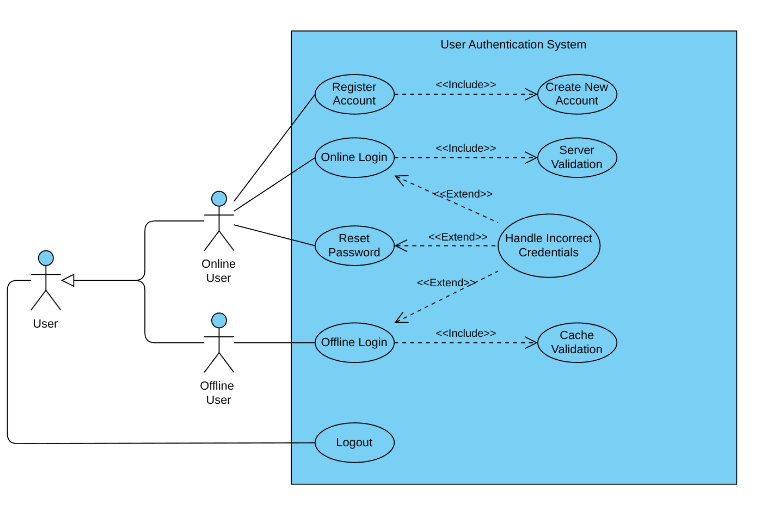
\includegraphics[width=0.9\textwidth]{registration_login.png}
  \caption{Registration and Login Use Case Diagram}
  \label{fig:reg-log-use-case}
\end{figure}

\subsection{Search Term Use Case Diagram}
\begin{figure}[H]
  \centering
  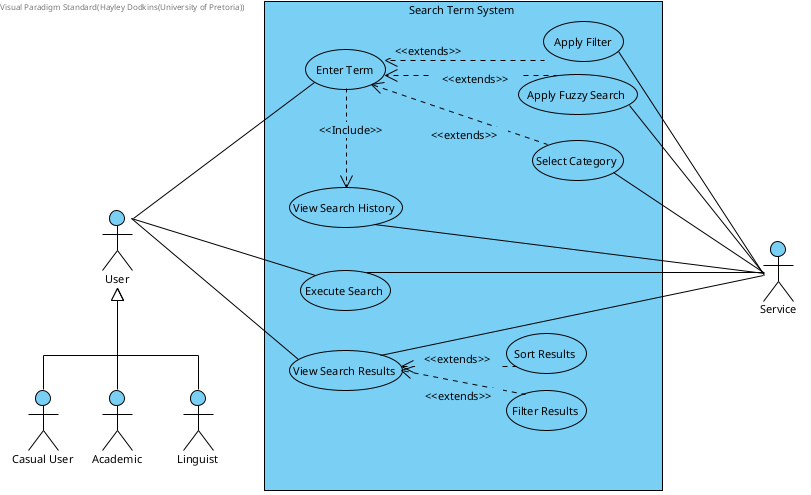
\includegraphics[width=0.9\textwidth]{SearchTermUseCase.png}
  \caption{Search Term Use Case Diagram for Mavito}
  \label{fig:search-use-case}
\end{figure}

\subsection{Gamification Use Case Diagram}
\begin{figure}[H]
  \centering
  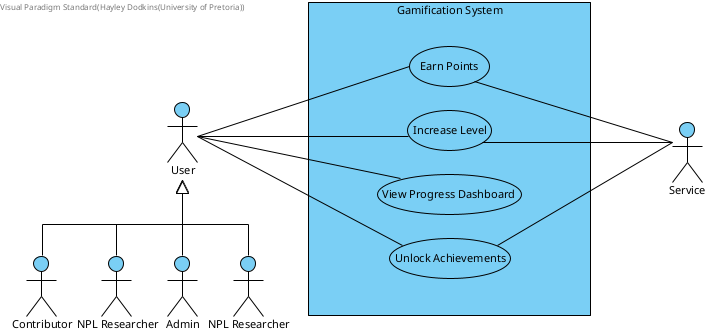
\includegraphics[width=0.9\textwidth]{GamifictionUseCase.png}
  \caption{Gamification Use Case Diagram}
  \label{fig:gamification-use-case}
\end{figure}

\subsection{Visualization Use Case Diagram}
\begin{figure}[H]
  \centering
  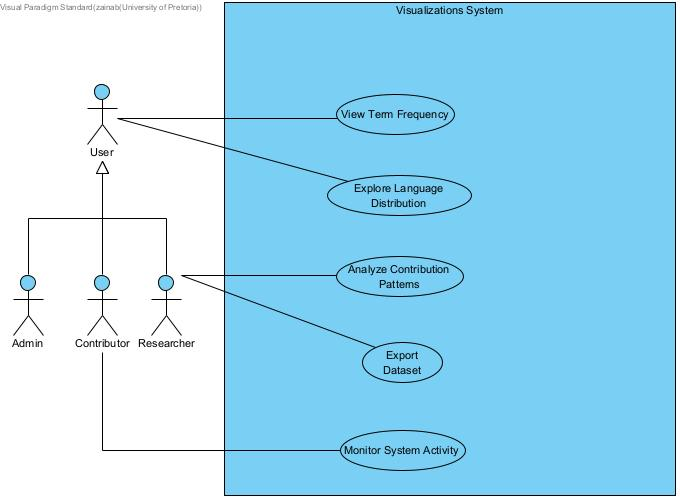
\includegraphics[width=0.9\textwidth]{Visualizations.jpg}
  \caption{Visualization Use Case Diagram}
  \label{fig:visualization-use-case}
\end{figure}

\subsection{Themes Use Case Diagram}
\begin{figure}[H]
  \centering
  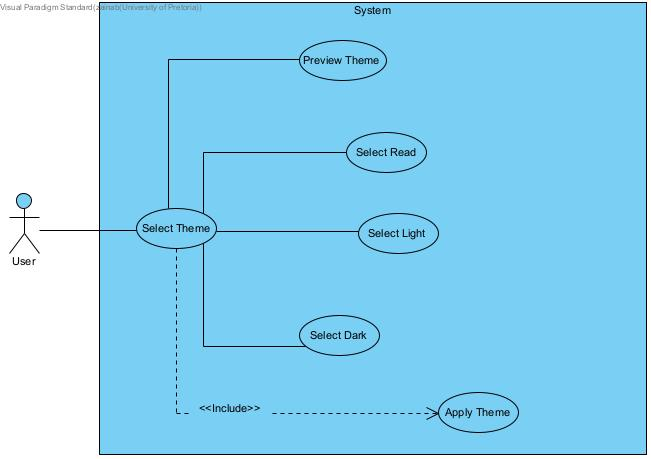
\includegraphics[width=0.9\textwidth]{Themes_UseCase.jpg}
  \caption{Themes Use Case Diagram}
  \label{fig:themes-use-case}
\end{figure}

\subsection{Contributions Use Case Diagram}
\begin{figure}[H]
  \centering
  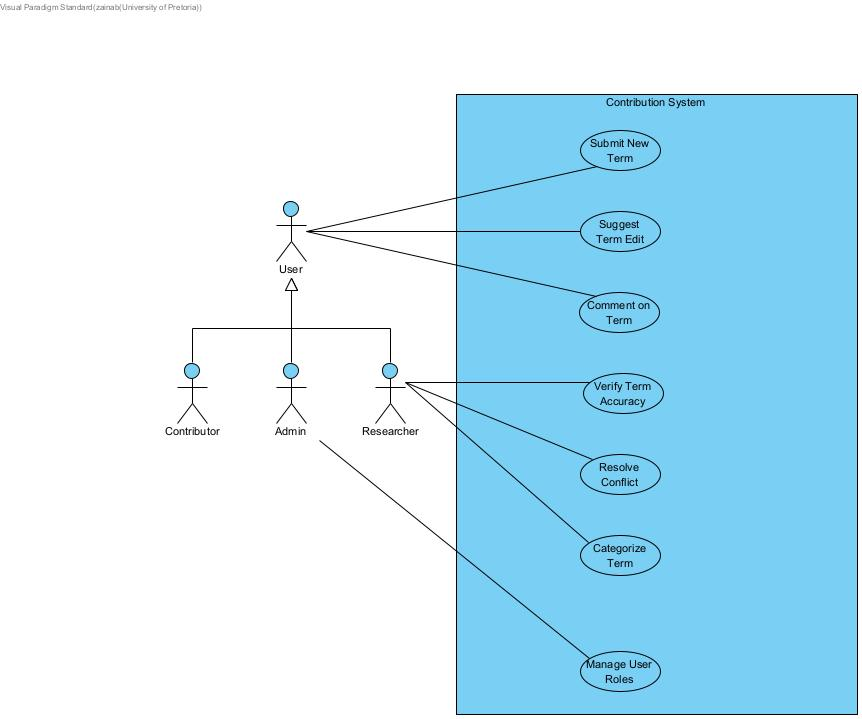
\includegraphics[width=0.9\textwidth]{Contributions.jpg}
  \caption{Contributions Use Case Diagram}
  \label{fig:contributions-use-case}
\end{figure}

\subsection{Overview}
The main use cases covered include:
\begin{itemize}
  \item Browsing and searching multilingual terms
  \item Earning contribution points through gamified interactions
  \item Registration and login ineractions
  \item User Contributions
  \item User themes
  \item Data visualizations
\end{itemize}


\section{Functional Requirements}

\begin{enumerate}[label=FR\arabic*:, leftmargin=2.5em]

    \item \textbf{Glossary Browsing and Search}
    \begin{itemize}
        \item FR1.1: The system shall allow users to browse available glossaries and term banks.
        \item FR1.2: The system shall provide a unified search interface across all multilingual glossaries.
        \item FR1.3: The system shall allow users to search for terms using exact matches, partial strings, or semantic similarity.
        \item FR1.4: The search results shall be ranked by relevance and display key metadata (definition, part of speech, language).
        \item FR1.5: The system shall highlight related terms and translations in the term view.
    \end{itemize}

    \item \textbf{Multilingual Support}
    \begin{itemize}
        \item FR2.1: The system shall support interface localization in multiple South African languages.
        \item FR2.2: The system shall allow users to switch the UI language at any time.
        \item FR2.3: The system shall correctly render special characters where applicable.
    \end{itemize}

    \item \textbf{User Contributions and Feedback}
    \begin{itemize}
        \item FR3.1: The system shall allow users to submit comments.
        \item FR3.2: The system shall allow users to submit corrections or suggestions for terms.
        \item FR3.3: The system shall send submitted feedback to a backend repository for moderation.
        \item FR3.4: The system shall support version control for submitted glossary data and prevent overwriting of validated entries.
        \item FR3.5: The system should be able to allow users to upvote/downvote term changes.
    \end{itemize}

    \item \textbf{AI-Enhanced Functionality}
    \begin{itemize}
        \item FR4.1: The system shall support AI-powered semantic search to retrieve conceptually related terms.
        \item FR4.2: The system may provide suggested definitions or translations using AI models.
        \item FR4.3: The system may automatically cluster terms based on meaning or domain.
        \item FR4.4: The system may auto-tag glossary entries with linguistic metadata (e.g., part-of-speech).
        \item FR4.5: The system may integrate with external NLP APIs for research purposes.
    \end{itemize}

    \item \textbf{Gamification}
    \begin{itemize}
        \item FR5.1: The system shall assign points to users when they submit valid suggestions, comments, or issue reports on glossary terms.
        \item FR5.2: The system shall track milestones based on user activity and unlock achievements or badges when predefined thresholds are reached.
        \item FR5.3: The system shall display a progress dashboard on the user's profile page, including total points, badges earned, and contribution rank.
        \item FR5.4: The system shall provide real-time feedback when users perform actions that affect their gamification status.
        \item FR5.5: The system shall support user rank or title progression as users accumulate points and reach specific contribution levels.
        \item FR5.6: The system shall queue gamified contributions made offline and synchronize them with the server once the user is reconnected.
        \item FR5.7: The system shall validate contributions before assigning gamification points to prevent abuse.
    \end{itemize}

    \item \textbf{Progressive Web Application Functionality}
    \begin{itemize}
        \item FR6.1: The system shall function as a PWA and be installable on mobile and desktop devices.
        \item FR6.2: The frontend shall use service workers to cache glossary data, enabling offline access to core features such as term lookup and browsing.
        \item FR6.3: The system shall store user feedback or contributions made offline and queue them for submission once connectivity is restored.
        \item FR6.4: The application shall automatically synchronize cached content with the server when an internet connection is detected.
        \item FR6.5: The system shall provide visual feedback or indicators when the app is operating in offline mode.
        \item FR6.6: The system shall support background updates of cached glossary data to maintain consistency with the server.
        \item FR6.8: The system shall allow users to download selected glossaries for offline access.
    \end{itemize}

    \item \textbf{Data Visualization and Analytics}
    \begin{itemize}
        \item FR7.1: The system should be able to display stats on word frequency and usage trends.
        \item FR7.2: The system should be able to visualize a user's contribution to different languages.
        \item FR7.3: The system should highlight trending words and new entries to the database.
        \item FR7.4: The system should be able to provide interactive charts or graphs for linguistic data.
    \end{itemize}

    \item \textbf{Data Import and Export}
    \begin{itemize}
        \item FR8.1: The system shall allow users to export glossary data in JSON format.
        \item FR8.2: The system shall allow users to export glossary data in CSV format.
        \item FR8.3: The system may allow authorized users to import glossaries in JSON or CSV format.
    \end{itemize}

\end{enumerate}


\section{Non-Functional Requirements}

\begin{enumerate}[label=NFR\arabic*:, leftmargin=2.5em]
    \item \textbf{Offline Accessibility}
    \begin{itemize}
        \item NFR1.1 The system shall support offline access to previously downloaded language resources.
        \item NFR1.2 The frontend shall use service workers and caching to allow uninterrupted use of core features without an active internet connection.
        \item NFR1.3 Synchronization of updated resources shall automatically occur once the device is back online.
    \end{itemize}
    
    \item \textbf{Performance and Responsiveness}
    \begin{itemize}
        \item NFR2.1 The system shall deliver fast search responses, with results displayed within 2 seconds for standard queries.
        \item NFR2.2 The frontend application shall load and become interactive within 3 seconds on devices with moderate hardware and average bandwidth.
        \item NFR2.3 UI interactions shall be smooth and not exceed 100ms latency where possible.
    \end{itemize}
    
    \item \textbf{Scalability}
    \begin{itemize}
        \item NFR3.1 The backend shall be able to handle simultaneous requests from a growing user base, including researchers and contributors.
        \item NFR3.2 The data architecture must accommodate the addition of new glossaries, languages, and APIs without the need for major refactoring.
    \end{itemize}
    
    \item \textbf{Security and Privacy}
    \begin{itemize}
        \item NFR4.1 All data transmissions between client and server shall be encrypted using HTTPS.
        \item NFR4.2 User-submitted feedback shall be sanitized and validated to prevent injection attacks.
        \item NFR4.3 The backend shall implement basic access control to restrict sensitive actions to authorized roles.
    \end{itemize}
    
    \item \textbf{Usability and Accessibility}
    \begin{itemize}
        \item NFR5.1 The user interface shall support all 11 official South African languages through dynamic localization.
        \item NFR5.2 The application shall conform to WCAG 2.1 Level AA accessibility guidelines to accommodate visually impaired users.
        \item NFR5.3 The system shall provide a clean and intuitive interface that requires no more than three clicks to reach key features.
    \end{itemize}
    
    \item \textbf{Maintainability}
    \begin{itemize}
        \item NFR6.1 The codebase shall follow modular and well-documented design practices to enable ease of maintenance.
        \item NFR6.2 The frontend and backend shall use consistent code formatting enforced via linting tools.
        \item NFR6.3 New contributors shall be able to understand and modify the codebase with minimal onboarding effort.
    \end{itemize}
    
    \item \textbf{Extensibility}
    \begin{itemize}
        \item NFR7.1 The system shall support the addition of new term banks and glossaries via a modular import system.
        \item NFR7.2 New frontend features shall be integrable without affecting the core application features.
        \item NFR7.3 The backend shall expose extensible REST API routes following OpenAPI standards.
    \end{itemize}
    
    \item \textbf{Reliability and Fault Tolerance}
    \begin{itemize}
        \item NFR8.1 The system shall gracefully handle failed API requests and notify the user when a feature is temporarily unavailable.
        \item NFR8.2 The frontend shall include fallback mechanisms for critical resources, ensuring minimal disruption in case of partial data loss.
        \item NFR8.3 The backend shall log all failed operations and expose logs for future debugging or auditing.
    \end{itemize}
    
    \item \textbf{Portability and Cross-Platform Compatibility}
    \begin{itemize}
        \item NFR9.1 The PWA shall work on major browsers (Chrome, Firefox, Edge, Safari) and platforms (Windows, Android, iOS, Linux).
        \item NFR9.2 The UI shall be fully responsive and usable on screen sizes ranging from smartphones to desktop monitors.
        \item NFR9.3 No feature shall be dependent on platform-specific behavior.
    \end{itemize}
    
    \item \textbf{Deployment and DevOps Readiness}
    \begin{itemize}
        \item NFR10.1 The backend shall be containerized using Docker to support consistent deployment across environments.
        \item NFR10.2 CI/CD pipelines shall be configured to run tests, build artifacts, and deploy the application to the cloud or GitHub Pages.
    \end{itemize}
\end{enumerate}


\section{Constraints}

\subsection{Overview}
This section outlines the constraints that govern the design, development, deployment, and maintenance of the \textbf{Mavito} application. These constraints stem from ethical considerations, client requirements, project context, budgetary limitations, and architectural guidelines. Adherence to these constraints is critical to the project's success and sustainability.

\subsection{Constraints}

\begin{enumerate}[label=2.\arabic*, leftmargin=2.5em]

    \item \textbf{Privacy and Data Minimization}
    \begin{itemize}
        \item The application must adopt a privacy-first approach.
        \item No personal user information may be collected unless voluntarily submitted.
        \item No personal data should be stored without explicit user consent.
        \item Any user data collected must comply with ethical research standards and university data policies.
        \item All stored data must follow ethical and data protection principles.
    \end{itemize}

    \item \textbf{Maintainability and Sustainability}
    \begin{itemize}
        \item The project must use a maintainable and reliable technology stack that future students or stakeholders can easily understand and extend.
        \item All source code must be well-documented, modular, and follow clean architecture principles.
        \item Technologies selected must have active community support and comprehensive documentation to minimize onboarding effort.
    \end{itemize}

    \item \textbf{Use of Open Source Technologies}
    \begin{itemize}
        \item Wherever possible, the project must use open-source frameworks and libraries.
        \item External packages or modules must have permissive licenses (e.g., MIT, Apache 2.0) and be cited appropriately.
    \end{itemize}

    \item \textbf{Budget Constraints}
    \begin{itemize}
        \item The project must be developed with minimal to zero cost.
        \item The team is not permitted to incur costs unless explicitly approved by the client.
        \item Hosting should utilize free tiers.
    \end{itemize}

    \item \textbf{Offline Functionality}
    \begin{itemize}
        \item The application must support offline access as a core feature.
        \item Core features must function without an active internet connection, using Progressive Web App (PWA) technologies such as service workers and local caching.
        \item Synchronization with the central repository must occur seamlessly once connectivity is restored.
    \end{itemize}

    \item \textbf{Version Control of Glossary Data}
    \begin{itemize}
        \item Glossary data and language resources must be version-controlled to prevent loss or corruption of validated content.
        \item User feedback must be stored separately and reviewed before merging into the main dataset.
        \item No glossary data may be overwritten without proper validation and versioning mechanisms.
    \end{itemize}

    \item \textbf{Ethical and Legal Considerations}
    \begin{itemize}
        \item No proprietary or restricted datasets may be used without explicit authorization.
        \item Contributions and authorship must be tracked where possible to preserve academic and community recognition.
    \end{itemize}

    \item \textbf{Performance and Efficiency}
    \begin{itemize}
        \item The application must be responsive and performant on low-resource or mobile devices.
        \item Heavy assets (e.g., large datasets or images) must be lazy-loaded or paginated.
        \item Search and filtering mechanisms must be optimized for performance on slower devices and large datasets.
    \end{itemize}

    \item \textbf{Accessibility Requirements}
    \begin{itemize}
        \item The application must adhere to WCAG 2.1 AA accessibility standards.
        \item Features such as text-to-speech, keyboard navigation, color contrast, and screen reader support should be considered where feasible.
        \item Dark mode and adjustable text size are encouraged to support visual diversity in users.
    \end{itemize}

    \item \textbf{Deployment and Portability}
    \begin{itemize}
        \item The system must be deployable using containerization to support ease of testing and reproducibility.
        \item CI/CD pipelines must be used for automated builds and testing.
        \item Both frontend and backend should be deployable without manual intervention.
    \end{itemize}

    \item \textbf{Multi-Language Support}
    \begin{itemize}
        \item The interface must support multiple South African languages.
        \item The system must be internationalization-ready using industry-standard practices (e.g., translation JSON files, locale selectors).
        \item UI elements, glossaries, and feedback must render correctly regardless of language.
    \end{itemize}

\end{enumerate}

\subsection{Summary}
These constraints serve as the foundation for all architectural, design, and implementation decisions made during the development of \textbf{Mavito}. They ensure the solution is ethical, sustainable, inclusive, affordable, and aligned with the client’s goals of making multilingual resources accessible to all.


\section{Domain Model}
\begin{figure}[H]
  \centering
  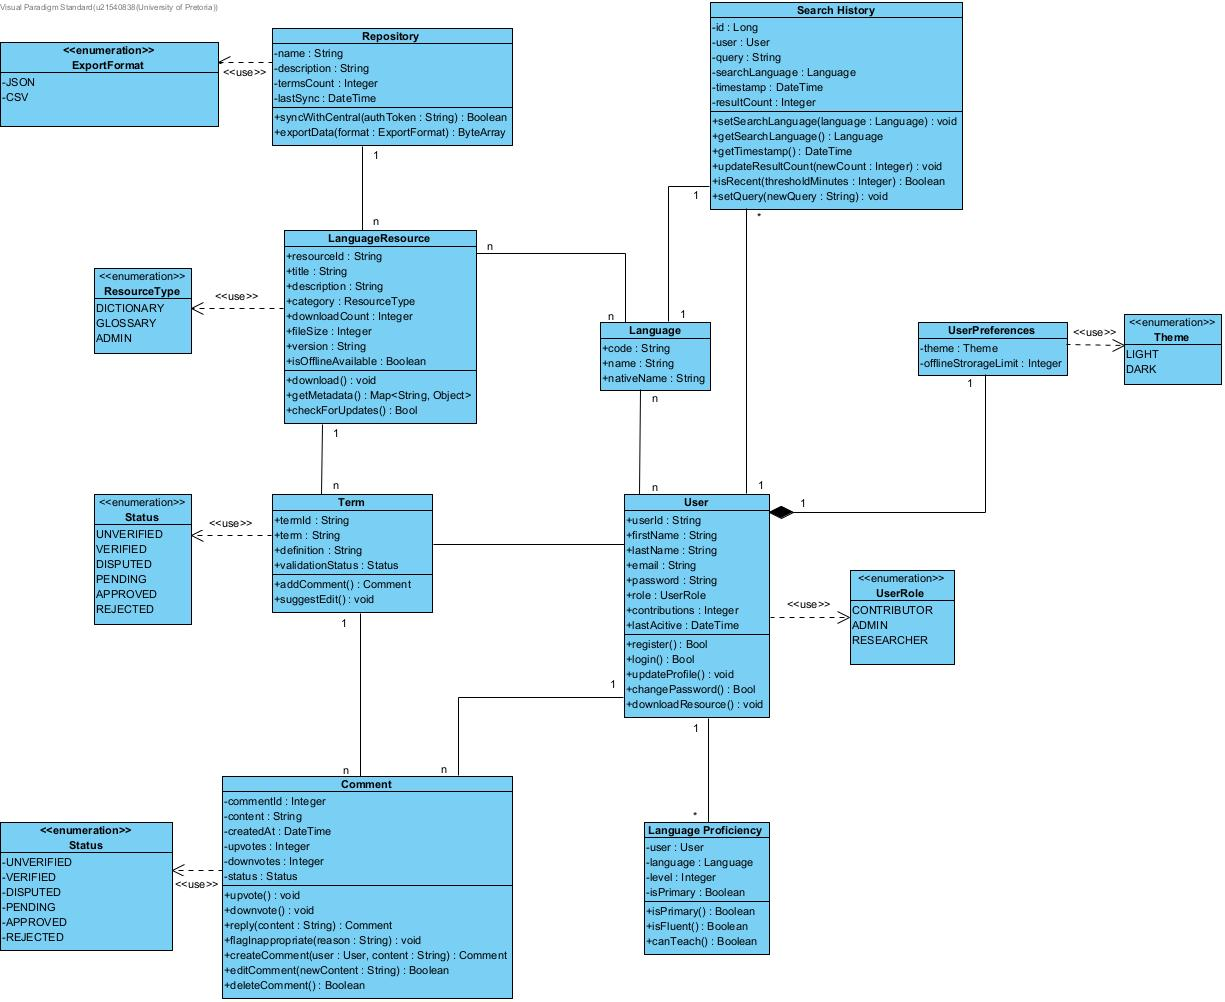
\includegraphics[width=0.9\textwidth]{domain_model.jpg}
  \caption{Domain Model}
  \label{fig:domain-model}
\end{figure}

\section{Architecture Patterns}
The architectural foundation of Mavito combines the Microkernel and Microservices patterns to address both extensibility and service independence. This hybrid approach is essential for building a maintainable, scalable, and community-driven multilingual terminology platform. Each pattern plays a distinct role in supporting the system’s goals, and their selection is justified below.

\subsection{Microkernel Pattern}
The Microkernel pattern is employed in the frontend and core backend logic to support feature modularity. The Mavito PWA core includes only essential functionality: multilingual glossary viewing, search, and feedback submission. Additional services such as AI-enhanced semantic search, gamification metrics, or user-uploaded terms implemented as optional plugins that extend the core without modifying it.
\newline
\textbf{Motivation and Usage:}
\begin{itemize}
    \item Allows teams to add or disable features without affecting the base system.
    \item Enables experimentation with novel features like gamified contribution scoring or data validation without bloating the core.
    \item No personal data should be stored without explicit user consent.
    \item Ideal for open-source collaboration where contributors might develop new plugins independently.
\end{itemize}

\subsection{Microservices Pattern}
On the backend, the system uses a Microservices architecture. Each core function is encapsulated within an independently deployable service. These services communicate via well-defined APIs, often exposed through REST endpoints.
\newline
\textbf{Motivation and Usage:}
\begin{itemize}
    \item Services like term search, user contribution tracking, and feedback moderation are implemented and deployed independently.
    \item Facilitates horizontal scaling where search and analytics services can scale independently of the glossary browser.
    \item Increases fault isolation as a failure in one service does not compromise the rest of the application.
    \item Supports technology diversity, enabling future services to be written in different languages.
\end{itemize}

\subsection{Benefits of the Combined Approach}
\begin{itemize}
    \item \textbf{Extensibility:} New features can be added as plugins without disrupting the rest of the system.
    \item \textbf{Separation of Concerns:} Responsibilities are clearly delineated between base functionality and modular enhancements.
    \item \textbf{Deployment Flexibility:} Dockerized services and a plugin-based UI allow different deployments to include only the relevant modules.
\end{itemize}
\newline
This combination ensures that Mavito remains agile, extensible, and robust, with clearly isolated responsibilities across its components. These are key traits for a system designed to support a growing multilingual terminology community.

\section{Design Patterns}

The Mavito system employs several proven design patterns to promote modularity, clarity, and maintainability. These patterns are used across both frontend and backend components to ensure clean separation of concerns, extensibility, and testability.

\subsection{Backend Design Patterns}

\begin{itemize}
    \item \textbf{Repository Pattern}: This pattern abstracts the data access layer, decoupling the application’s business logic from its persistence mechanisms. In Mavito, this is used to isolate FastAPI routes from direct interaction with JSON files or potential databases. This makes it easier to substitute or refactor storage formats later.

    \item \textbf{Service Layer Pattern}: This pattern encapsulates business logic in service classes rather than embedding it in route handlers. For example, the glossary service processes user input, validates term entries, and formats responses. This keeps the FastAPI route functions minimal and focused on HTTP handling.

    \item \textbf{Proxy Pattern}: Used to control access to sensitive glossary data, this pattern allows features like lazy-loading or permission-based access control. For instance, the proxy layer can prevent unreviewed user-uploaded data from being merged directly into the main glossary.

    \item \textbf{Adapter Pattern}: This is used to integrate external APIs, particularly AI/NLP tools for semantic search or text analytics into the system without modifying the core glossary services. Adapters provide a uniform interface so different NLP services can be swapped in or out easily.

    \item \textbf{Builder Pattern}: Glossary term responses often contain complex nested structures (e.g., term, translations, part of speech, examples, contributor metadata). The builder pattern helps assemble these objects step-by-step, ensuring clarity and consistency in API responses.
\end{itemize}

\subsection{Frontend Design Patterns}

\begin{itemize}
    \item \textbf{Observer Pattern}: React’s reactive rendering model naturally supports this pattern. In Mavito, UI components subscribe to state changes such as term updates, language switching, or sync status. This enables real-time UI updates without manual DOM manipulation.

    \item \textbf{Model–View–Controller (MVC)}: Mavito uses React components as Views, application state as the Model, and event handlers or hooks as Controllers. This separation ensures testable, reusable components and a clear flow of data and control.

    \item \textbf{Model–View–ViewModel (MVVM)}: For more complex UI flows, especially those with async behavior or derived state (e.g., loading indicators, sync status), Mavito uses custom React hooks as ViewModels to isolate logic from presentation. This allows clean and declarative UIs while keeping logic reusable across components.
\end{itemize}
\newline
Together, these patterns ensure that both backend services and frontend components remain modular, understandable, and adaptable to future requirements. They also enable team members to work in parallel with minimal friction.


\section{Technology Requirements}
The Mavito system is built using modern, open-source technologies selected for their performance, maintainability, and compatibility with offline-first web applications and modular architectures. These technologies are categorized below according to their role in the stack.
\subsection{Frontend}
\begin{itemize}
  \item \textbf{Framework:} React (via Vite) for fast, modular UI development.
  \item \textbf{Language:} TypeScript for type safety and developer productivity.
  \item \textbf{Styling:} SCSS modules and Tailwind CSS for flexible and responsive design.
  \item \textbf{Build Tool:} Vite for fast local development and optimized production builds.
  \item \textbf{PWA Features:} Service workers and localStorage/IndexedDB for offline capabilities.
  \item \textbf{Testing:} Vitest for unit testing; Cypress for end-to-end testing.
  \item \textbf{Linting and Formatting:} ESLint and Prettier for code consistency.
  \item \textbf{Pre-commit Hooks:} Husky for running ESLint and Prettier on staged files, and for enforcing commit message conventions.
\end{itemize}

\subsection{Backend}
\begin{itemize}
  \item \textbf{Framework:} FastAPI for high-performance, Pythonic web APIs.
  \item \textbf{Language:} Python 3.11 with Pydantic for validation and typing.
  \item \textbf{Service Model:} Microservices organized by function.
  \item \textbf{Database:} PostgreSQL.
  \item \textbf{API Documentation:} FastAPI automatically generates OpenAPI-compliant service contracts, which are accessible via a ReDoc interface. This provides structured, human-readable API documentation derived directly from the backend codebase and Pydantic models.
  \item \textbf{Linting:} Ruff for fast, extensible linting.
  \item \textbf{Static Type Checking:} Mypy to ensure type correctness.
  \item \textbf{Formatting:} Black for consistent code formatting.
  \item \textbf{Testing:} Pytest for integration and unit tests.
  \item \textbf{Cloud Platform:} Google cloud for hosting.
\end{itemize}

\subsection{DevOps and Deployment}
\begin{itemize}
  \item \textbf{Containerization:} Docker for consistent development and deployment environments.
  \item \textbf{Orchestration:} Docker Compose for local service management.
  \item \textbf{CI/CD:} GitHub Actions for automated linting, testing, and deployment.
  \item \textbf{Hosting:} GitHub Pages.
\end{itemize}

\section{Service Contracts}
\begin{itemize}
Stub
\end{itemize}

\end{document}
